\section{Evaluation} \label{evalsec}
Optimizing code to use special techniques does not ensure that the final code will run faster than the original code. For this reason, the following section will look into what is gained and what is lost by each optimization type. The primary evaluation will be on CPU cycles and cycle/instruction ratio, as timed benchmarks would possibly yield unreliable results., due to overhead between the communicating parties (especially the possible overhead of the extra computation done by the test environment). Asking for cycles and instruction used on the \texttt{PQ-VexRiscV} CPU is easily done using a Hardware Abstraction Layer that exposes a \texttt{c} API with exactly this functionality (plus some).
\begin{figure}[t]
    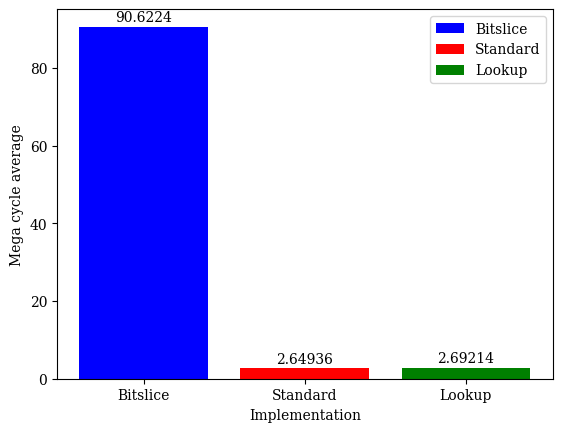
\includegraphics[width=0.5\textwidth]{resources/bar_avg_cycle.png}
    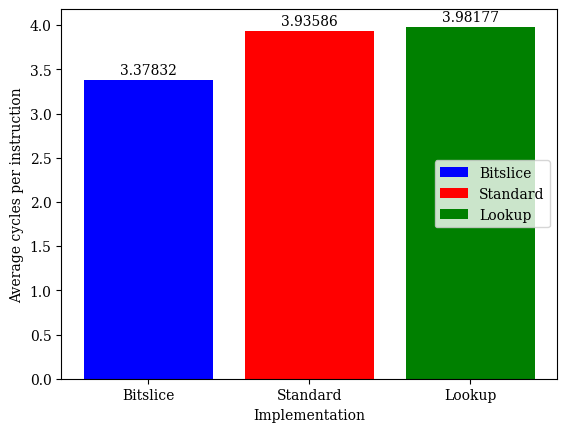
\includegraphics[width=0.5\textwidth]{resources/bar_avg_ratio.png}
    \caption{The figure to the left is the amount of mega cycles on average over 10 tests and the one on the right is the average cycles per instructions over the same 10 tests.}
    \label{eval:cycle}
\end{figure}
\subsection{Testing platform}
The three implementations listed in \cref{eval:cycle} were benchmarked on a platform with
\begin{description}
    \item \textbf{Processor}: PQVexRiscV
    \item \textbf{Speed}: \textbf{1.44 DMIPS/Mhz?}
    \item \textbf{Memory}: 512kB of RAM and 512kB of ROM
\end{description}
which in turn was simulated on
\begin{description}
    \item \textbf{Processor}: Ryzen 7 5800X
    \item \textbf{Operating System}: Linux 5.12.6-arch1-1
    \item \textbf{GCC}: riscv64-unknown-elf-gcc v. 10.2.0, with the \texttt{-O3} flag
    \item \textbf{Verilator}: Version 4.102
\end{description}
\subsection{Performance of the Reference Implementation}
Much of the focus for the reference implementation and its optimizations rely on instructions provided by the x86 or ARM ISAs. This is clear from the \cite{rainbownist} as was described in \cref{implementation:ffa}. As can be seen on the left in \cref{eval:cycle}, the standard implementation uses (estimated) $2.64936$ mega cycles to do a verification on the RISC-V platform. Comparing these numbers to the 30 to 42 kilo cycles used by the Intel platforms (classic Rainbow, level I) given in \cite{rainbownist}, the less complex structure of RISC-V has quite an increase in cycles used. However, as those platforms are all desktop- or server-grade hardware and two of the three processors make use of Intels AVX2 instruction-set, a comparison of this sort does not state much.
\medskip\\
In \cite{rainbownist} the implementation was also tested on an ARM Cortex-M4 for which this RISC-V CPU has more similar purposes to than an x86 platform. For the Cortex-M4, their implementation uses 238 kilo cycles for classical Rainbow with Security level I. This number is still quite a lot smaller than the 2.6 mega cycles on this implementation.
\subsection{Performance of the Lookup Table Implementation}
The lookup table implementation performs relatively well in relation to the standard implementation. From the left part of \cref{eval:cycle} the lookup table implementation can be seen to use around 400 kilo cycles more than the standard implementation did. As the relative performance between the standard implementation and the tests in \cite{rainbownist} was shown to be quite largely in favor of the platforms tested in \cite{rainbownist}, this variant did not help yield a better comparative result.
\medskip\\
The same is true for the cycles per instruction ratio, as it is very close to being the same as the standard implementation. The difference is around 1.17\%. To be sure that these 1.17\% in difference are constant and not coincidence, further testing would be needed.
\medskip\\
To come closer to the goal of obtaining a more efficient computational method for verifying Rainbow signatures, it is possible that a purely lookup table variant might be a bit quicker. Including the SIMD extension for RISC-V might help do the optimizations that the original authors used with regard to AVX2 instruction set and \texttt{TBL}. Further research could be made into alternative schemes of computing the public map, to see which scheme benefits from the additional 256 bytes from this table and whether or not this would incur a beneficial performance boost.
\medskip\\
Provided this minimal slowdown in performance and the 512 kB of RAM and ROM storage, 256 bytes might not be a significant amount of extra storage to use. However, this does not outweigh the performance difference between the standard implementation and this. Looking into the memory usage differences between the two implementations should be done for any conclusive answers on this.
\subsection{Performance of the Bitsliced Implementation}
The reasoning behind trying a bitsliced computational technique for verification is that it has the potential to do very fast nearly constant-time computations. As can be seen in the left part of \cref{eval:cycle}, this is not the case. The percentage increase in the amount of cycles used were around 3320\%, which is quite significant. Given the conditions of this project and my experience on this front, this is with very high probability a programmer-induced error somewhere in the bitslicing implementation. These specific results should for this reason not be seen as conclusive.
\medskip\\
An interesting outcome, which can potentially be carried onto a better bitslicing implementation, is that the cycles per instruction is lower than that of the standard and lookup table implementations. This decrease in the ratio of cycles per instruction corresponds to around a 14\% decrease. As the bitsliced implementation makes use of many simple instructions like \texttt{and}, \texttt{xor} and \texttt{not} it is not unlikely that these are the reason for the lower ratio. Given a potentially simpler set of instructions used (using fewer cycles each) these changes could potentially see a better overall performance should the ratio carry on.
\medskip\\
Improving the bitslicing approach could nonetheless be done by including some RISC-V assembly code, in which the amount of instructions used can also be more clear. Doing this, however, does not yield a platform independent approach as the current one is, so further research could go two ways from here. Either looking into the problems of the current pure \texttt{c} bitslicing and improving it, or looking into how to optimize instruction counts by injecting at least some RISC-V assembly.
\medskip\\
The bitslicing scheme in itself is not a bad way of obtaining faster code, as was shown in \cite{betterbitslicer}. In that paper, the clock cycle count was decreased from 1619 and 3529 kilo cycles to 239 and 238 kilo cycles in the case of verification. The cycle counts before optimization are very clearly close to what can be seen by the standard implementation in \cref{eval:cycle}.